\documentclass[10pt, aspectratio=169]{beamer}

% --------------------------------------------------------------------------- %
% Theme
% --------------------------------------------------------------------------- %
\usetheme{Madrid}
\usecolortheme{whale}
\setbeamertemplate{navigation symbols}{}

\setbeamertemplate{itemize item}{\textbullet}
\setbeamertemplate{itemize subitem}{$\circ$}
\setbeamertemplate{itemize subsubitem}{$\blacktriangleright$}
\setbeamercolor{itemize item}{fg=black}
\setbeamercolor{itemize subitem}{fg=black}
\setbeamercolor{itemize subsubitem}{fg=black}

\definecolor{best}{RGB}{198, 239, 206}
\definecolor{accent}{RGB}{0, 60, 113}

% --------------------------------------------------------------------------- %
% Packages
% --------------------------------------------------------------------------- %
\usepackage{booktabs}
\usepackage{graphicx}
\usepackage{amsmath}
\usepackage{amssymb}
\usepackage{colortbl}
\usepackage{array}

\graphicspath{{figures/}}

% --------------------------------------------------------------------------- %
% Metadata
% --------------------------------------------------------------------------- %
\title[Few-Shot Classification]{Fine-tuning the Foundational Model for Image Classification using Few Samples}
\subtitle{}
\author[Gundapu \& Nandan]{
  \textbf{Gundapu Nitish Kumar} \quad \textbf{Mourya Nandan} \\[0.18cm]
  \small CS 6350: Computer Vision \quad TPA-17 \\[0.04cm]
  \small CSE Department
}
\institute[IITM]{IIT Madras}
\date{\today}

\begin{document}

% --------------------------------------------------------------------------- %
% 1. Title
% --------------------------------------------------------------------------- %
\begin{frame}[plain]
  \titlepage
\end{frame}

% --------------------------------------------------------------------------- %
% 2. References and acknowledgements
% --------------------------------------------------------------------------- %
\begin{frame}[t]{References \& Acknowledgements}
  \begin{columns}[T]
    \begin{column}{0.64\textwidth}
      {\scriptsize
      \begin{enumerate}
        \setlength{\itemsep}{1pt}
        \item A. Dosovitskiy et al., ``An Image is Worth 16$\times$16 Words: Transformers for Image Recognition at Scale,'' \emph{ICLR}, 2021.
        \item O. Sim\'eoni et al., ``DINOv3,'' \emph{arXiv}, 2025.
        \item E. J. Hu et al., ``LoRA: Low-Rank Adaptation of Large Language Models,'' \emph{ICLR}, 2022.
        \item E. Ben Zaken, Y. Goldberg, S. Ravfogel, ``BitFit: Simple Parameter-efficient Fine-tuning for Transformer-based Masked Language-models,'' \emph{ACL}, 2022.
        \item R. R. Selvaraju et al., ``Grad-CAM: Visual Explanations from Deep Networks via Gradient-based Localization,'' \emph{ICCV}, 2017.
        \item L. van der Maaten, G. Hinton, ``Visualizing Data using t-SNE,'' \emph{JMLR}, 2008.
        \item M.-E. Nilsback, A. Zisserman, ``Automated Flower Classification over a Large Number of Classes,'' \emph{ICVGIP}, 2008.
        \item O. M. Parkhi et al., ``Cats and Dogs,'' \emph{CVPR}, 2012.
      \end{enumerate}}
    \end{column}
    \begin{column}{0.34\textwidth}
      \begin{block}{Acknowledgements}
        \footnotesize
        \begin{itemize}
          \item Google ViT-B/16 checkpoint; Meta DINOv3 checkpoint via \texttt{timm}
          \item PyTorch, PyTorch Lightning, Hugging Face Transformers, PEFT, \texttt{timm}, scikit-learn
          \item NVIDIA RTX PRO 4000 Blackwell (24\,GB) for all runs
          \item Used AITool (Deepseek-v4-flash) for Boiler Plate Code Generation and Documentation
        \end{itemize}
      \end{block}
    \end{column}
  \end{columns}
\end{frame}

% --------------------------------------------------------------------------- %
% 3. Problem statement
% --------------------------------------------------------------------------- %
\begin{frame}[t]{Problem Statement}
  \begin{alertblock}{TPA-17 brief}
    \small
    To evaluate and compare fine-tuning strategies on foundation models (CLIP, DINOv2, ViT) for a downstream image classification task in a domain with limited labeled data. The project explores fine-tuning and adapter-based methods (e.g., LoRA) for optimal performance and resource trade-offs.
  \end{alertblock}

  \vspace{0.15cm}
  \begin{columns}[T]
    \begin{column}{0.55\textwidth}
      \small
      \textbf{Scope taken in this study}
      \begin{itemize}
        \item Two image-only foundation models: ViT-B/16 and DINOv3-B/16.
        \item Two fine-grained, limited-label datasets: Flowers102 and Oxford-IIIT Pet.
        \item Five strategies: full fine-tuning, linear probing (LP), LoRA, BitFit, and training-free nearest-class-mean (NCM).
        \item Compare accuracy, precision, recall, F1, trainable parameters, time, and GPU memory.
      \end{itemize}
    \end{column}
    \begin{column}{0.42\textwidth}
      \small
      \textbf{Questions}
      \begin{enumerate}
        \item Does a strong pretrained representation need full fine-tuning?
        \item How much accuracy survives when $<1\%$ of the parameters move?
        \item When is a training-free prototype classifier enough?
      \end{enumerate}
    \end{column}
  \end{columns}
\end{frame}

% --------------------------------------------------------------------------- %
% 4. Datasets and configurations
% --------------------------------------------------------------------------- %
\begin{frame}[t]{Datasets \& Configurations}
  \centering
  \small
  \setlength{\tabcolsep}{5pt}
  \begin{tabular}{lcc}
    \toprule
    & \textbf{Flowers102} & \textbf{Oxford-IIIT Pet} \\
    \midrule
    Classes & 102 flower species & 37 cat/dog breeds \\
    Images & 8{,}189 & 7{,}349 (3{,}680 train + 3{,}669 test) \\
    Train split & 510 (5/class, from 1{,}020) & 370 (10/class, from 3{,}680) \\
    Validation & 1{,}020 (official) & 735 (20\% of test, stratified) \\
    Test split & 6{,}149 (official) & 2{,}934 (remaining 80\%) \\
    Input resolution & $224\times224$ (ViT) & $224\times224$ (ViT) \\
                       & $256\times256$ (DINOv3) & $256\times256$ (DINOv3) \\
    \bottomrule
  \end{tabular}

  \vspace{0.25cm}
  \begin{columns}[T]
    \begin{column}{0.52\textwidth}
      \footnotesize
      \textbf{Protocol}
      \begin{itemize}
        \item Seed 42; deterministic, class-stratified splits.
        \item Fixed label budget: \textbf{5 images/class} on Flowers102 and \textbf{10 images/class} on Pet (510 and 370 training images).
        \item Augmentation: RandomResizedCrop (scale 0.65--1.0), horizontal flip, model-specific normalization.
        \item No colour jitter, keeping the comparison close to a standard linear-probe protocol.
      \end{itemize}
    \end{column}
    \begin{column}{0.45\textwidth}
      \begin{block}{Why these datasets?}
        \footnotesize
        Frozen features are already strong on Flowers102, so it isolates the low-label regime. Oxford-IIIT Pet is harder: 37 fine-grained breeds, large pose/background variation, and visible cat/dog confusion.
      \end{block}
    \end{column}
  \end{columns}
\end{frame}

% --------------------------------------------------------------------------- %
% 5. Flowers102 examples
% --------------------------------------------------------------------------- %
\begin{frame}[t]{Flowers102: 102 Fine-Grained Species}
  \centering
  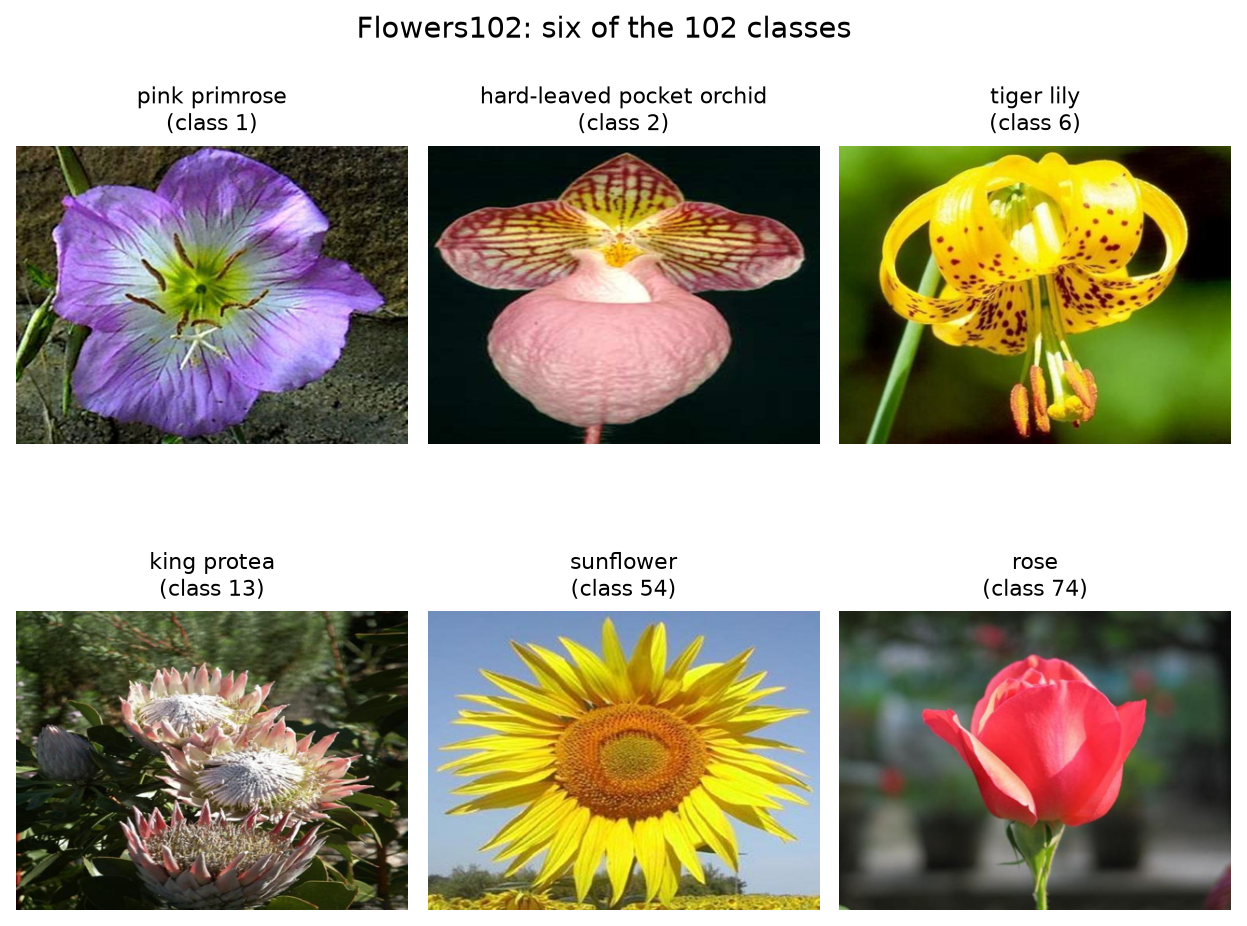
\includegraphics[width=0.94\linewidth,height=0.68\textheight,keepaspectratio]{flowers_samples.png}
  \vspace{-0.12cm}
  {\footnotesize
  \begin{itemize}
    \item Fine-grained differences in petal shape, colour, and inflorescence; backgrounds, scale, and illumination vary widely.
    \item The official training split contains only \textbf{10 images per class}; each run trains on a deterministic \textbf{5-image-per-class} subset.
  \end{itemize}}
\end{frame}

% --------------------------------------------------------------------------- %
% 6. Oxford-IIIT Pet examples
% --------------------------------------------------------------------------- %
\begin{frame}[t]{Oxford-IIIT Pet: 37 Cat and Dog Breeds}
  \centering
  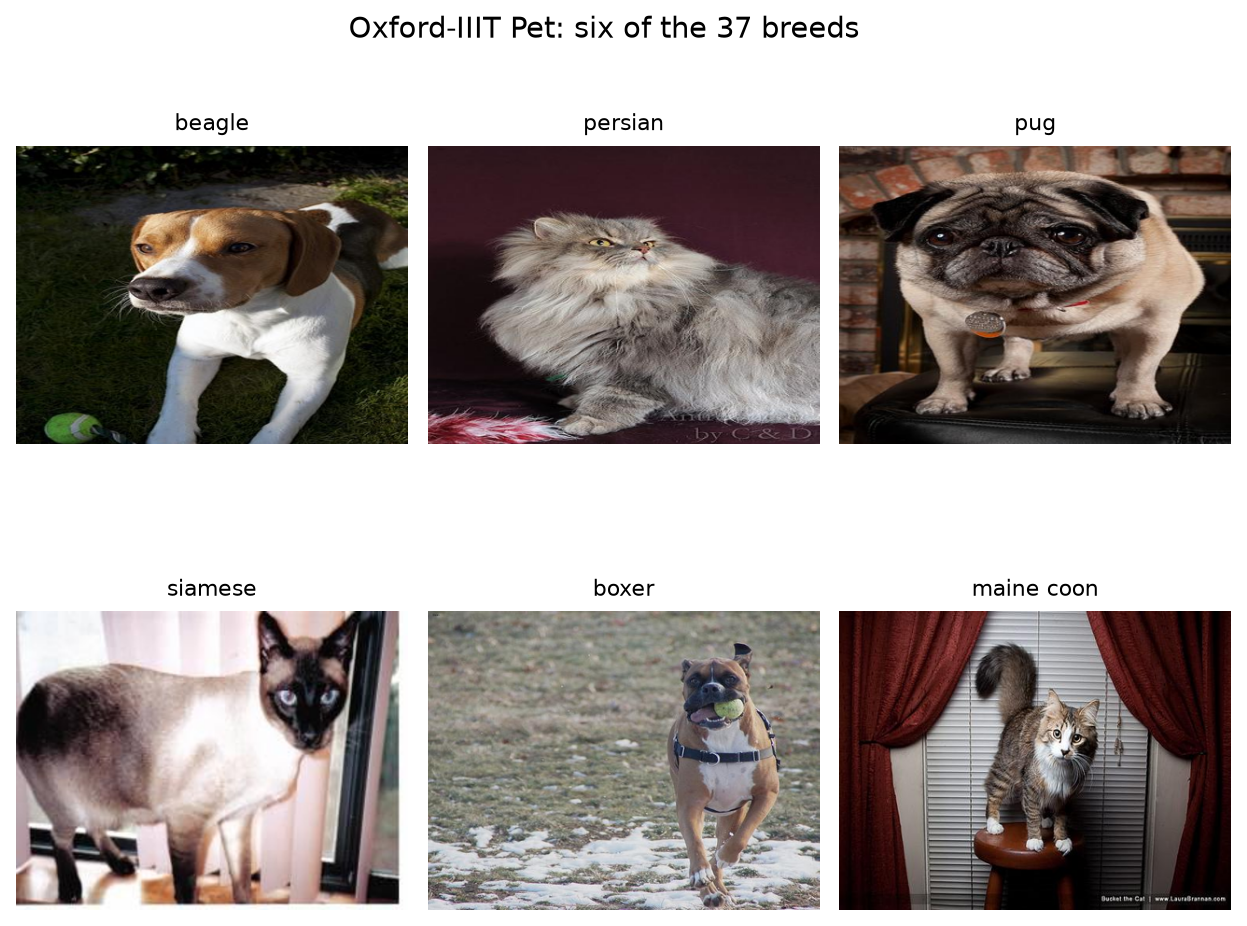
\includegraphics[width=0.94\linewidth,height=0.68\textheight,keepaspectratio]{pet_samples.png}
  \vspace{-0.12cm}
  {\footnotesize
  \begin{itemize}
    \item 25 dog and 12 cat breeds; roughly 200 images per class, with large intra-class variation in pose, coat, and background. Each run trains on \textbf{10 images per class}.
    \item Visually similar breeds and cat/dog confusion make Pet substantially harder than Flowers102 for frozen features.
  \end{itemize}}
\end{frame}

% --------------------------------------------------------------------------- %
% 7. Model architectures
% --------------------------------------------------------------------------- %
\begin{frame}[t]{Model Architectures: ViT-B/16 and DINOv3-B/16}
  \begin{columns}[T]
    \begin{column}{0.49\textwidth}
      \centering
      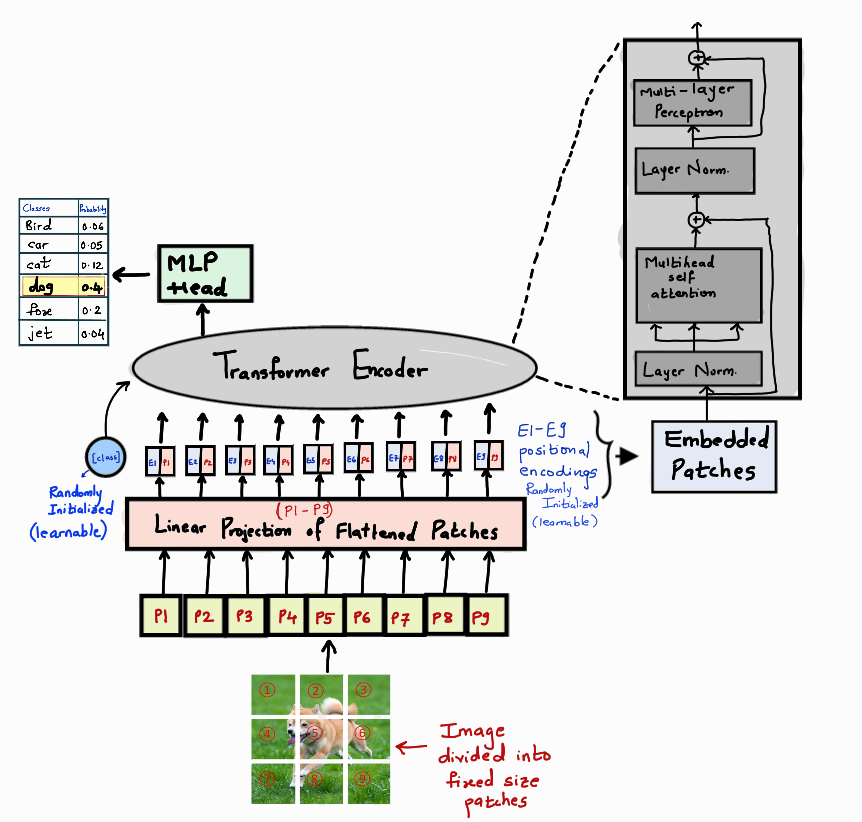
\includegraphics[width=\linewidth,height=0.37\textheight,keepaspectratio]{vit_arch.png}
      \vspace{-0.1cm}
      {\footnotesize
      \begin{itemize}
        \item \textbf{ViT-B/16}: 12 transformer layers, width 768, 12 heads, $16\times16$ patches, $224\times224$ input.
        \item Supervised ImageNet pretraining (\texttt{google/vit-base-patch16-224}); CLS token feeds the linear head.
        \item 85.9M parameters in total.
      \end{itemize}}
    \end{column}
    \begin{column}{0.49\textwidth}
      \centering
      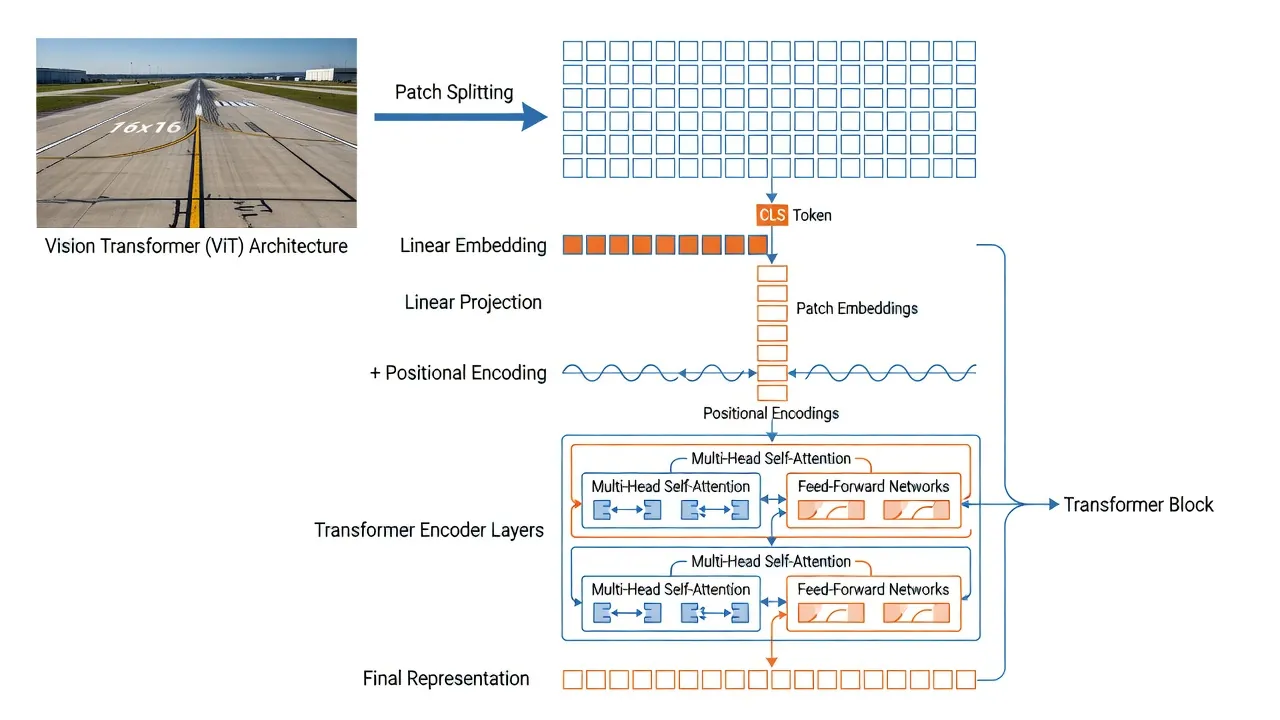
\includegraphics[width=\linewidth,height=0.37\textheight,keepaspectratio]{dino_v3.png}
      \vspace{-0.1cm}
      {\footnotesize
      \begin{itemize}
        \item \textbf{DINOv3-B/16}: ViT-B/16 backbone trained with self-supervised DINOv3 on LVD-1689M.
        \item $256\times256$ input, CLS token plus 4 register tokens, rotary position encoding; CLS token feeds the head.
        \item 85.7M parameters in total.
      \end{itemize}}
    \end{column}
  \end{columns}

  \vspace{0.05cm}
  {\footnotesize \textbf{Shared recipe:} replace the classifier with a $C$-way head; only the trainable parameter set changes.}
\end{frame}

% --------------------------------------------------------------------------- %
% 7b. End-to-end pipeline diagram
% --------------------------------------------------------------------------- %
\begin{frame}[t]{End-to-End Training and Evaluation Pipeline}
  \centering
  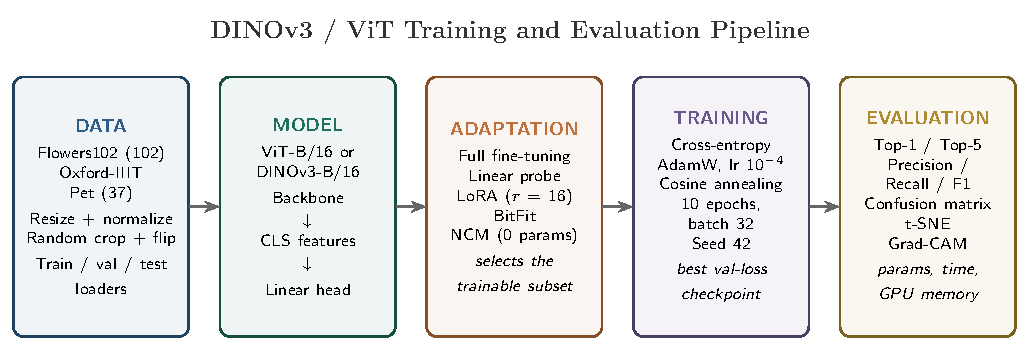
\includegraphics[width=0.97\linewidth]{fig_pipeline_diagram.pdf}
  \vspace{0.05cm}
  {\footnotesize
  \begin{itemize}
    \item The five stages are shared by ViT and DINOv3; only the backbone and LoRA target modules differ.
    \item The adaptation stage controls which parameters are trainable; NCM skips the training stage entirely.
    \item Every run writes predictions, per-class F1, confusion matrices, t-SNE embeddings, and Grad-CAM maps.
  \end{itemize}}
\end{frame}

% --------------------------------------------------------------------------- %
% 8. Methods (1/2)
% --------------------------------------------------------------------------- %
\begin{frame}[t]{Adaptation Strategies (1/2): How Many Weights Move?}
  \small
  \begin{description}
    \item[Full fine-tuning] Update the backbone $\theta$ and the head $\phi$. Most expressive, most expensive; 85.9M (ViT) or 85.7M (DINOv3) trainable parameters.
    \item[Linear probing (LP)] Freeze $\theta$, train only the head $\phi$. Trainable: 78{,}438 parameters on Flowers102 and 28{,}453 on Pet (0.03--0.09\% of the model).
    \item[Nearest-class-mean (NCM)] No optimisation. Compute one L2-normalised prototype per class from the frozen CLS features:
  \end{description}

  \[
    \mu_c = \frac{1}{|\mathcal{S}_c|}\sum_{i\in\mathcal{S}_c}
    \frac{f_\theta(x_i)}{\lVert f_\theta(x_i)\rVert_2},
    \qquad
    \hat{y} = \arg\max_c \cos\!\big(f_\theta(x), \mu_c\big).
  \]

  \vspace{-0.15cm}
  \begin{columns}[T]
    \begin{column}{0.48\textwidth}
      \begin{block}{NCM in the few-label regime}
        \footnotesize
        One prototype per class is estimated from just 5 (Flowers102) or 10 (Pet) labelled images; no optimiser, no epochs, no checkpoint selection.
      \end{block}
    \end{column}
    \begin{column}{0.48\textwidth}
      \begin{block}{Cost of NCM}
        \footnotesize
        Zero trainable parameters and a single feature-extraction pass: 6.6--12.8\,s and 0.62--0.70\,GB at evaluation time.
      \end{block}
    \end{column}
  \end{columns}

  \vspace{0.1cm}
  \footnotesize
  All methods use the same cross-entropy objective and the same data order; only the trainable parameter mask differs, and NCM trains nothing at all.
\end{frame}

% --------------------------------------------------------------------------- %
% 9. Methods (2/2)
% --------------------------------------------------------------------------- %
\begin{frame}[t]{Adaptation Strategies (2/2): BitFit, LoRA, and the Parameter Budget}
  \begin{columns}[T]
    \begin{column}{0.52\textwidth}
      \small
      \textbf{BitFit.} Freeze every weight matrix; train all bias terms in the backbone plus the full classification head. This updates 0.12--0.21\% of the model.
      \vspace{0.15cm}

      \textbf{LoRA.} Freeze the backbone and insert low-rank updates $\Delta W = BA$ into the attention projections. Rank $r=16$, $\alpha=32$, dropout 0.1; the head is also trained.
      \vspace{0.15cm}

      \begin{block}{LoRA target modules}
        \footnotesize
        ViT (Hugging Face): \texttt{q\_proj}, \texttt{v\_proj} \\
        DINOv3 (\texttt{timm}): \texttt{attn.qkv}, \texttt{attn.proj}
      \end{block}
      \begin{block}{Why low rank?}
        \footnotesize
        The adaptation is expected to be low-dimensional: LoRA trains 0.62--0.96M parameters (0.7--1.1\%) while leaving the pretrained representation almost untouched.
      \end{block}
    \end{column}
    \begin{column}{0.46\textwidth}
      \centering
      \scriptsize
      \setlength{\tabcolsep}{2.5pt}
      \begin{tabular}{lcccc}
        \toprule
        & \multicolumn{2}{c}{\textbf{ViT-B/16}} & \multicolumn{2}{c}{\textbf{DINOv3-B/16}} \\
        \cmidrule(lr){2-3}\cmidrule(lr){4-5}
        Method & Flowers & Pet & Flowers & Pet \\
        \midrule
        Full & 85.88M & 85.83M & 85.72M & 85.67M \\
             & (100\%) & (100\%) & (100\%) & (100\%) \\
        LP & 78.4k & 28.5k & 78.4k & 28.5k \\
           & (0.09\%) & (0.03\%) & (0.09\%) & (0.03\%) \\
        LoRA & 668k & 618k & 963k & 913k \\
             & (0.77\%) & (0.72\%) & (1.11\%) & (1.06\%) \\
        BitFit & 181k & 131k & 154k & 104k \\
               & (0.21\%) & (0.15\%) & (0.18\%) & (0.12\%) \\
        \rowcolor{best}
        NCM & 0 & 0 & 0 & 0 \\
            & (0\%) & (0\%) & (0\%) & (0\%) \\
        \bottomrule
      \end{tabular}

      \vspace{0.15cm}
      {\tiny Trainable parameters (fraction of the full model).}
    \end{column}
  \end{columns}
\end{frame}

% --------------------------------------------------------------------------- %
% 10b. Adapter strategies summary (from the report, Table II)
% --------------------------------------------------------------------------- %
\begin{frame}[t]{Adapter Strategies: Which Parameters Move?}
  \centering
  {\scriptsize ``Yes'' marks components the optimiser updates; ``No'' marks frozen or unused components.}

  \vspace{0.2cm}
  \resizebox{\textwidth}{!}{%
  \renewcommand{\arraystretch}{1.22}
  \begin{tabular}{@{}lcccccc@{}}
    \toprule
    \textbf{Strategy} & \textbf{Backbone weights} & \textbf{Backbone biases} & \textbf{LoRA adapters} & \textbf{Classifier head} & \textbf{Optimizer} & \textbf{Trainable params} \\
    \midrule
    Full fine-tuning & Yes & Yes & No & Yes & Yes & 85.7--85.9M (100\%) \\
    Linear probing & No & No & No & Yes & Yes & 28k--78k (0.03--0.09\%) \\
    LoRA & No & No & Yes & Yes & Yes & 0.62--0.96M (0.7--1.1\%) \\
    BitFit & No & Yes & No & Yes & Yes & 104k--181k (0.12--0.21\%) \\
    \rowcolor{best}
    NCM & No & No & No & No$^{\dagger}$ & No & 0 \\
    \midrule
    \multicolumn{7}{@{}l}{$^{\dagger}$NCM computes class prototypes from frozen features; the head is not used for classification.} \\
    \bottomrule
  \end{tabular}}

  \vspace{0.55cm}
  \begin{columns}[T]
    \begin{column}{0.49\textwidth}
      \begin{block}{What this matrix says}
        \footnotesize
        Only four parameter groups are ever updated: backbone weights, backbone biases, LoRA adapters, and the head. Every strategy is a different subset of this matrix.
      \end{block}
    \end{column}
    \begin{column}{0.49\textwidth}
      \begin{block}{Budget span}
        \footnotesize
        Full fine-tuning updates 100\% of the model (85.7--85.9M). LP, LoRA, and BitFit update only 0.03--1.11\%, and NCM updates nothing.
      \end{block}
    \end{column}
  \end{columns}
\end{frame}

% --------------------------------------------------------------------------- %
% 10c. Training configuration
% --------------------------------------------------------------------------- %
\begin{frame}[t]{Training Configuration for the Four Trained Methods}
  \begin{columns}[T]
    \begin{column}{0.47\textwidth}
      \small
      \setlength{\tabcolsep}{4pt}
      \begin{tabular}{ll}
        \toprule
        \textbf{Setting} & \textbf{Value} \\
        \midrule
        Optimizer & AdamW \\
        Learning rate & $10^{-4}$ (all methods) \\
        Weight decay & 0.05 \\
        Schedule & cosine annealing \\
        Batch size & 32 \\
        Epochs & 20 \\
        \bottomrule
      \end{tabular}
    \end{column}
    \begin{column}{0.51\textwidth}
      \small
      \setlength{\tabcolsep}{4pt}
      \begin{tabular}{ll}
        \toprule
        \textbf{Setting} & \textbf{Value} \\
        \midrule
        Seed & 42 \\
        Precision & FP32 \\
        Checkpoint selection & lowest validation loss \\
        Early stopping & patience 10 (not triggered) \\
        Augmentation & RRC (0.65--1.0) + HFlip \\
        Hardware & RTX PRO 4000, 24\,GB \\
        \bottomrule
      \end{tabular}
    \end{column}
  \end{columns}

  \vspace{0.25cm}
  \begin{block}{Important details}
    \footnotesize
    \begin{itemize}
      \item The four trained methods share the \emph{same} optimiser, learning rate, schedule, epochs, and batch size; only the trainable parameter set differs.
      \item Fixed label budget: 5 images/class on Flowers102 and 10 images/class on Pet (510 and 370 training images).
      \item NCM has no optimiser and no epochs: it is a single feature-extraction pass followed by prototype assignment.
      \item The best checkpoint is selected on validation loss.
    \end{itemize}
  \end{block}
\end{frame}

% --------------------------------------------------------------------------- %
% 12. ViT / Flowers102
% --------------------------------------------------------------------------- %
\begin{frame}[t]{ViT-B/16 on Flowers102: Optimisation Traces}
  \centering
  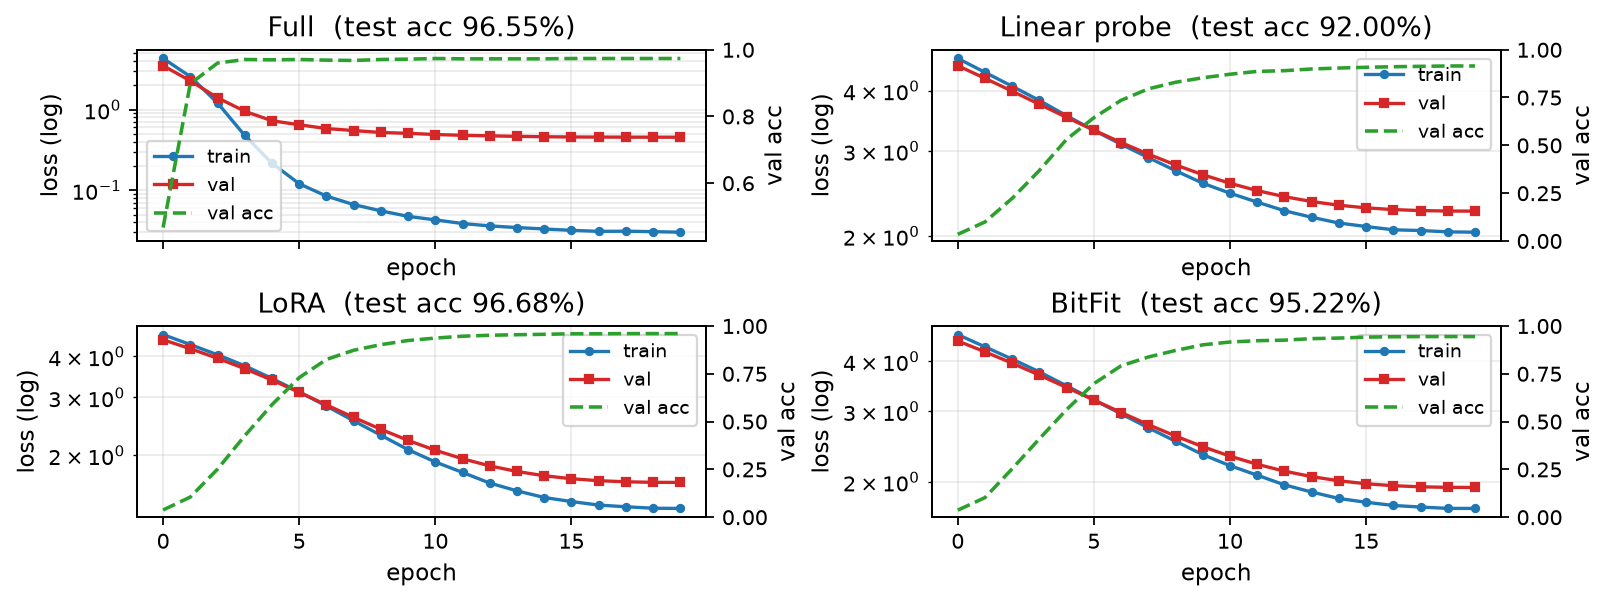
\includegraphics[width=\linewidth]{loss_vit_flowers102.png}
  \vspace{-0.15cm}
  {\footnotesize
  \begin{itemize}
    \item \textbf{Full} converges fastest in loss: val loss 0.455, val accuracy 97.35\%, test accuracy 96.55\%.
    \item \textbf{LP} is weakest but far from collapsing (92.00\% test, val loss 2.25); \textbf{LoRA} (96.68\%) and \textbf{BitFit} (95.22\%) beat it by 3.2--4.7 points. All trained runs pick epoch 19.
  \end{itemize}}
\end{frame}

% --------------------------------------------------------------------------- %
% 12. ViT / Pet
% --------------------------------------------------------------------------- %
\begin{frame}[t]{ViT-B/16 on Oxford-IIIT Pet: Optimisation Traces}
  \centering
  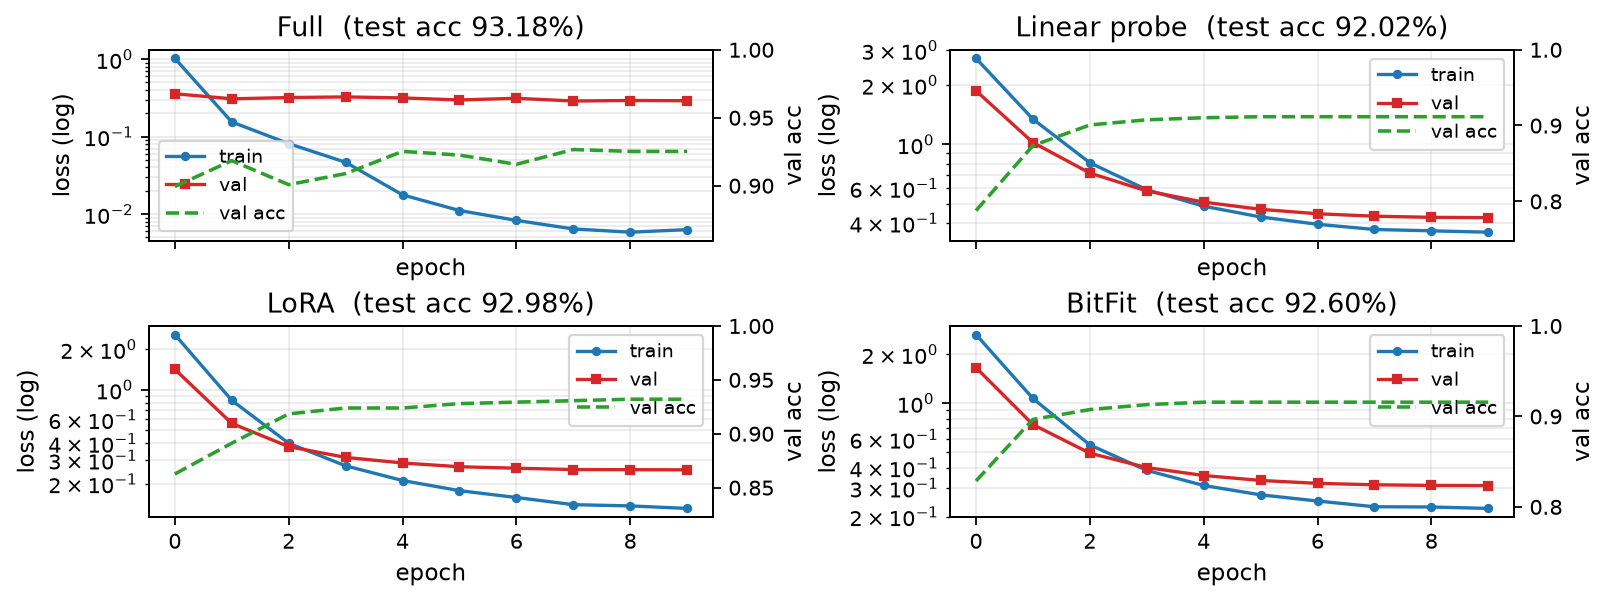
\includegraphics[width=\linewidth]{loss_vit_oxfordiiitpet.png}
  \vspace{-0.15cm}
  {\footnotesize
  \begin{itemize}
    \item \textbf{Full}: 88.10\% test / 87.89\% val (val loss 0.610), selected at epoch 19 like the other trained runs.
    \item \textbf{LoRA} is the best parameter-efficient method (86.61\%), only 1.5 points behind Full; \textbf{LP} is weakest at 81.15\%, with BitFit at 84.19\%.
  \end{itemize}}
\end{frame}

% --------------------------------------------------------------------------- %
% 13. DINOv3 / Flowers102
% --------------------------------------------------------------------------- %
\begin{frame}[t]{DINOv3-B/16 on Flowers102: Optimisation Traces}
  \centering
  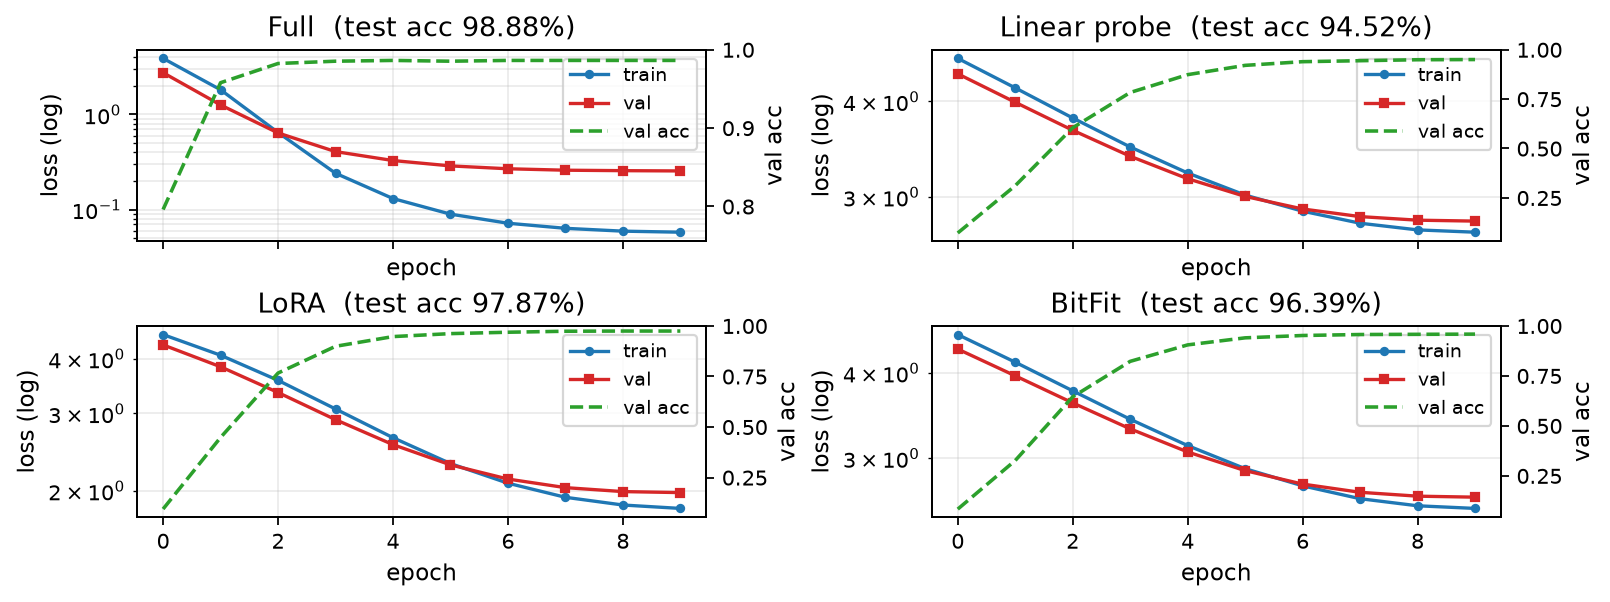
\includegraphics[width=\linewidth]{loss_dino_v3_flowers102.png}
  \vspace{-0.15cm}
  {\footnotesize
  \begin{itemize}
    \item \textbf{Full}: 97.01\% test / 97.45\% val (val loss 0.455); train loss falls to 0.046.
    \item \textbf{LoRA} (96.39\%) and \textbf{BitFit} (95.40\%) are close behind and beat \textbf{LP} (93.72\%); \textbf{NCM} (not shown) is training-free and best at 99.71\%.
  \end{itemize}}
\end{frame}

% --------------------------------------------------------------------------- %
% 14. DINOv3 / Pet
% --------------------------------------------------------------------------- %
\begin{frame}[t]{DINOv3-B/16 on Oxford-IIIT Pet: Optimisation Traces}
  \centering
  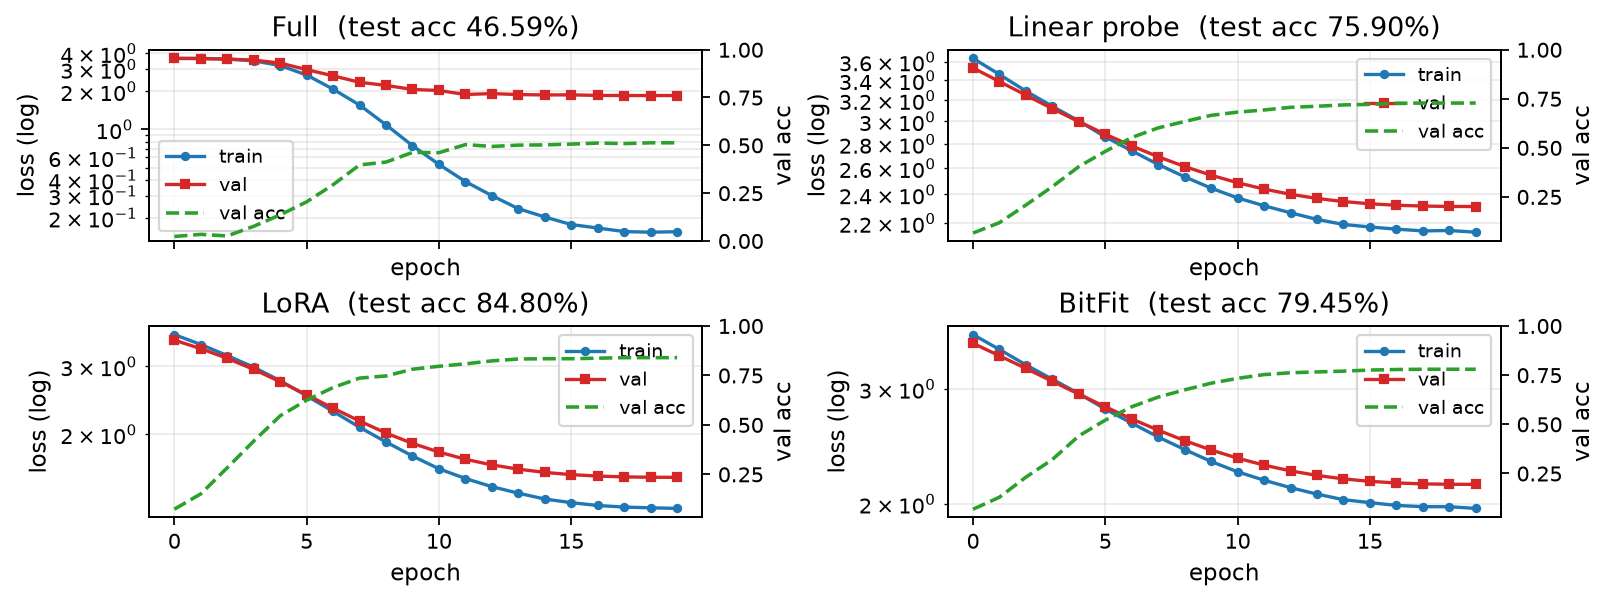
\includegraphics[width=\linewidth]{loss_dino_v3_oxfordiiitpet.png}
  \vspace{-0.32cm}
  {\footnotesize
  \begin{itemize}
    \item \textbf{Full fine-tuning overfits}: 46.59\% test / 50.88\% val, with train loss 0.156 vs val loss 1.85; its best checkpoint is epoch 17.
    \item \textbf{LoRA} is the best trained method (84.80\%), ahead of BitFit (79.45\%) and LP (75.90\%); \textbf{NCM} reaches 93.69\% on the frozen features.
  \end{itemize}}
\end{frame}

% --------------------------------------------------------------------------- %
% 15. Evaluation metrics table
% --------------------------------------------------------------------------- %
\begin{frame}[t]{Evaluation Metrics: Precision, Recall, F1, and Accuracy}
  \centering
  {\tiny Cell shading = best value in that column for the dataset. All numbers are percentages on the held-out test split.}

  \vspace{0.12cm}
  \begin{columns}[T]
    \begin{column}{0.49\textwidth}
      \centering
      {\scriptsize \textbf{ViT-B/16}} \\[0.05cm]
      \scriptsize
      \setlength{\tabcolsep}{2.6pt}
      \begin{tabular}{llcccc}
        \toprule
        Method & Data & Prec & Rec & F1 & Acc \\
        \midrule
        Full & Flowers & 96.14 & 97.61 & 96.74 & 96.55 \\
        LP & Flowers & 90.33 & 91.50 & 90.33 & 92.00 \\
        LoRA & Flowers & 95.86 & 96.65 & 96.07 & 96.68 \\
        BitFit & Flowers & 93.91 & 94.78 & 93.88 & 95.22 \\
        NCM & Flowers & \cellcolor{best}97.99 & \cellcolor{best}98.46 & \cellcolor{best}98.15 & \cellcolor{best}98.44 \\
        \midrule
        Full & Pet & 88.27 & 88.00 & 87.79 & 88.10 \\
        LP & Pet & 81.53 & 81.05 & 80.95 & 81.15 \\
        LoRA & Pet & 87.07 & 86.55 & 86.47 & 86.61 \\
        BitFit & Pet & 84.43 & 84.11 & 83.97 & 84.19 \\
        NCM & Pet & \cellcolor{best}91.85 & \cellcolor{best}91.45 & \cellcolor{best}91.40 & \cellcolor{best}91.48 \\
        \bottomrule
      \end{tabular}
    \end{column}
    \begin{column}{0.49\textwidth}
      \centering
      {\scriptsize \textbf{DINOv3-B/16}} \\[0.05cm]
      \scriptsize
      \setlength{\tabcolsep}{2.6pt}
      \begin{tabular}{llcccc}
        \toprule
        Method & Data & Prec & Rec & F1 & Acc \\
        \midrule
        Full & Flowers & 96.91 & 97.53 & 97.11 & 97.01 \\
        LP & Flowers & 93.06 & 93.42 & 92.50 & 93.72 \\
        LoRA & Flowers & 96.18 & 96.70 & 96.19 & 96.39 \\
        BitFit & Flowers & 94.65 & 94.92 & 94.33 & 95.40 \\
        NCM & Flowers & \cellcolor{best}99.65 & \cellcolor{best}99.71 & \cellcolor{best}99.66 & \cellcolor{best}99.71 \\
        \midrule
        Full & Pet & 47.14 & 46.49 & 45.98 & 46.59 \\
        LP & Pet & 77.77 & 75.87 & 75.34 & 75.90 \\
        LoRA & Pet & 86.16 & 84.75 & 84.51 & 84.80 \\
        BitFit & Pet & 81.17 & 79.42 & 78.94 & 79.45 \\
        NCM & Pet & \cellcolor{best}93.66 & \cellcolor{best}93.57 & \cellcolor{best}93.50 & \cellcolor{best}93.69 \\
        \bottomrule
      \end{tabular}
    \end{column}
  \end{columns}

  \vspace{0.12cm}
  {\tiny Top-5 accuracy is 80.67--99.93\% across all 20 runs; macro precision, recall, and F1 are unweighted means over classes.}
\end{frame}

% --------------------------------------------------------------------------- %
% 16. Confusion matrices
% --------------------------------------------------------------------------- %
\begin{frame}[t]{Confusion Matrices: Where the Remaining Errors Live}
  \centering
  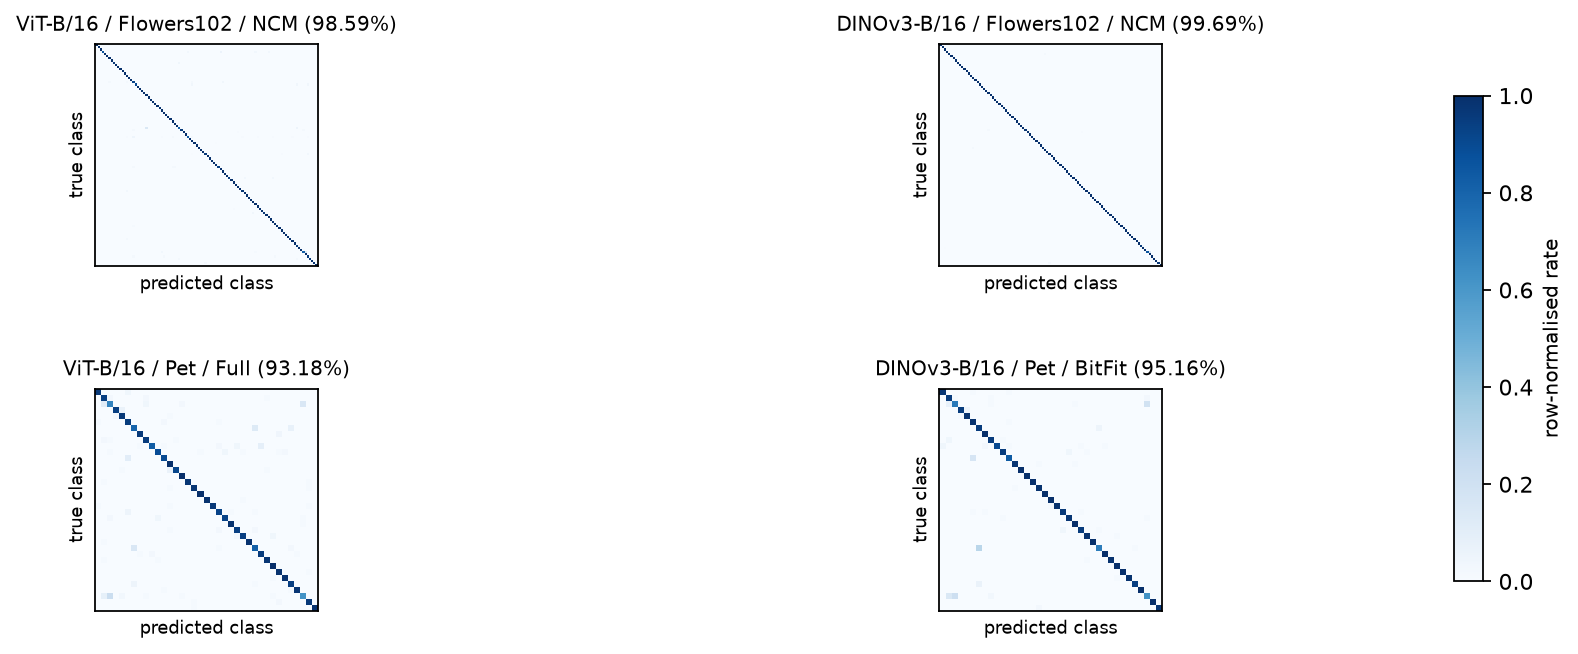
\includegraphics[width=0.86\linewidth]{confusion_grid.png}
  \vspace{-0.15cm}
  {\footnotesize
  \begin{itemize}
    \item \textbf{Flowers102}: the NCM diagonal is almost clean (ViT 98.44\%, DINOv3 99.71\%); remaining errors are between visually similar species.
    \item \textbf{Oxford Pet}: off-diagonal cat/dog and breed confusions; DINOv3 NCM is best (93.69\%) and ViT Full reaches 88.10\%. The trained DINOv3 methods trail NCM by 9--21 points, so the Pet/DINOv3 panel shows NCM. Matrices are row-normalised (diagonal = per-class recall).
  \end{itemize}}
\end{frame}

% --------------------------------------------------------------------------- %
% 17. Grad-CAM
% --------------------------------------------------------------------------- %
\begin{frame}[t]{Grad-CAM: What the Models Look At}
  \centering
  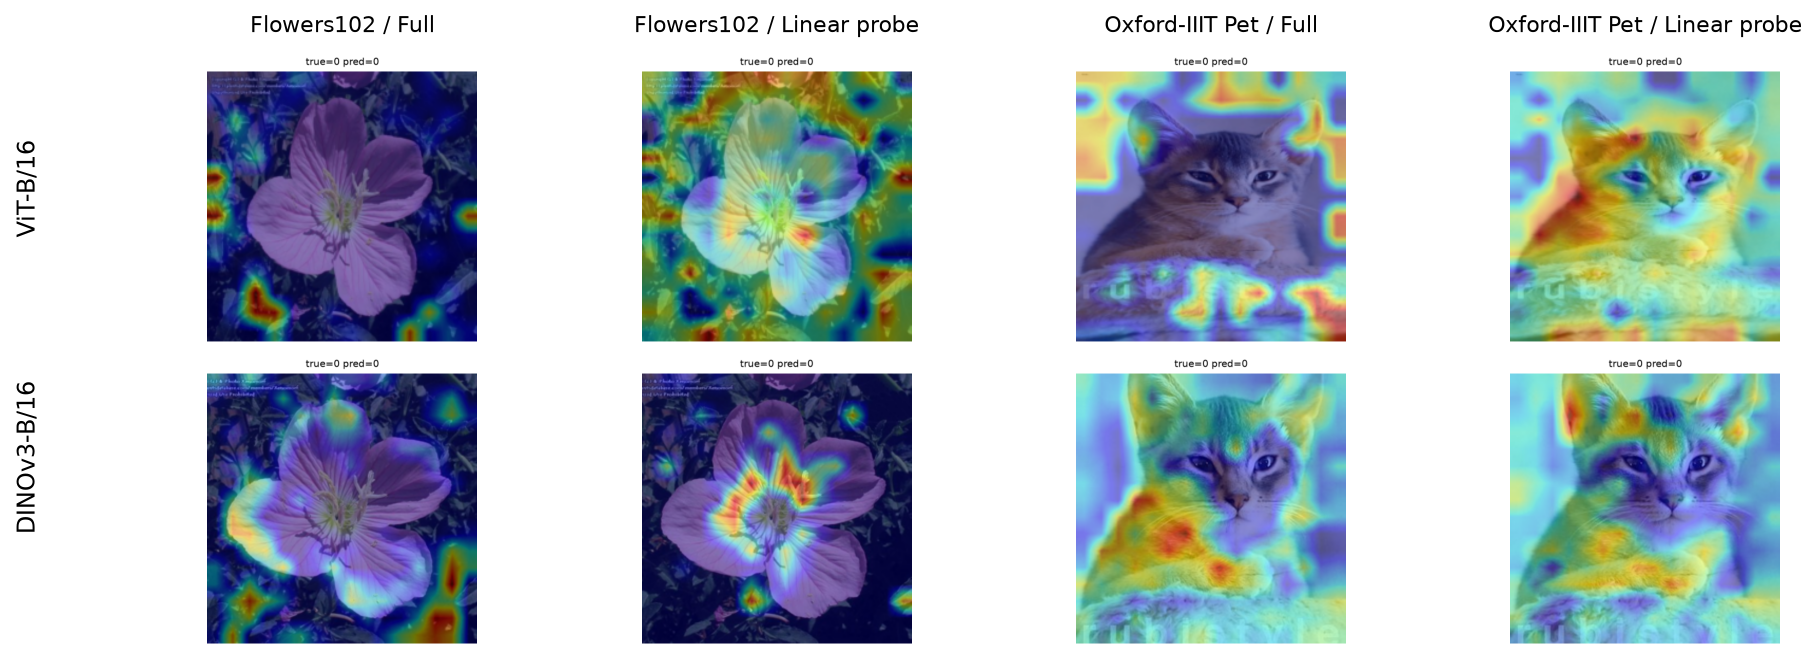
\includegraphics[width=0.95\linewidth]{gradcam_examples.png}
  \vspace{-0.18cm}
  {\footnotesize
  \begin{itemize}
    \item ViT maps are localized on petals, faces, and object parts; DINOv3 maps are broader and more object-centric.
    \item Linear probing often spreads attention more than full fine-tuning on the ViT examples; DINOv3 maps stay broad in both.
    \item ViT uses the final block, DINOv3 the penultimate block (final-block patch gradients vanish); NCM has no gradients, so no Grad-CAM.
  \end{itemize}}
\end{frame}

% --------------------------------------------------------------------------- %
% 18. t-SNE: ViT
% --------------------------------------------------------------------------- %
\begin{frame}[t]{t-SNE Maps: ViT-B/16}
  \centering
  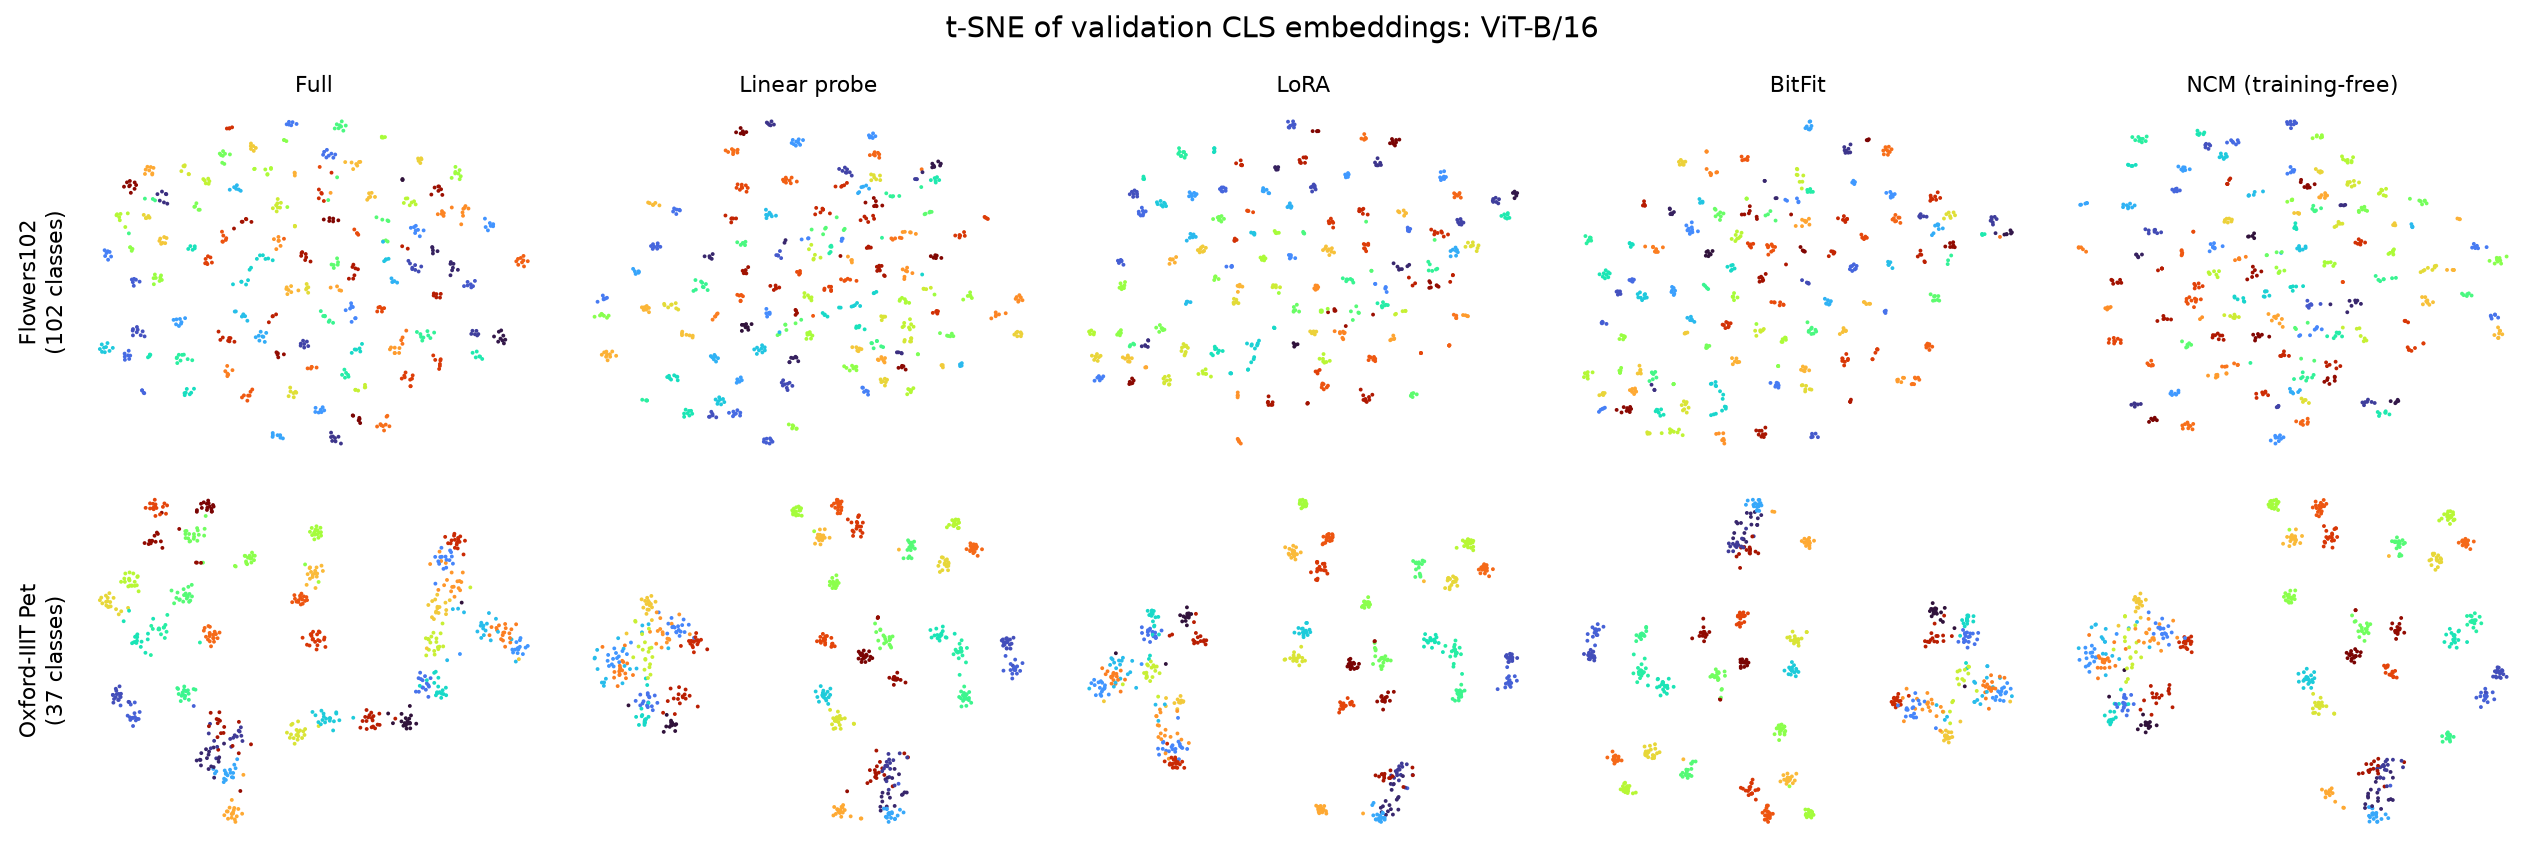
\includegraphics[width=\linewidth]{tsne_vit.png}
  \vspace{-0.18cm}
  {\footnotesize
  \begin{itemize}
    \item Flowers102 forms separable clusters even in the frozen-feature panels, consistent with NCM at 98.44\%.
    \item On Pet the frozen features separate breeds clearly, yet the LP head reaches only 81.15\%; the head, not the representation, remains the bottleneck.
  \end{itemize}}
\end{frame}

% --------------------------------------------------------------------------- %
% 19. t-SNE: DINOv3
% --------------------------------------------------------------------------- %
\begin{frame}[t]{t-SNE Maps: DINOv3-B/16}
  \centering
  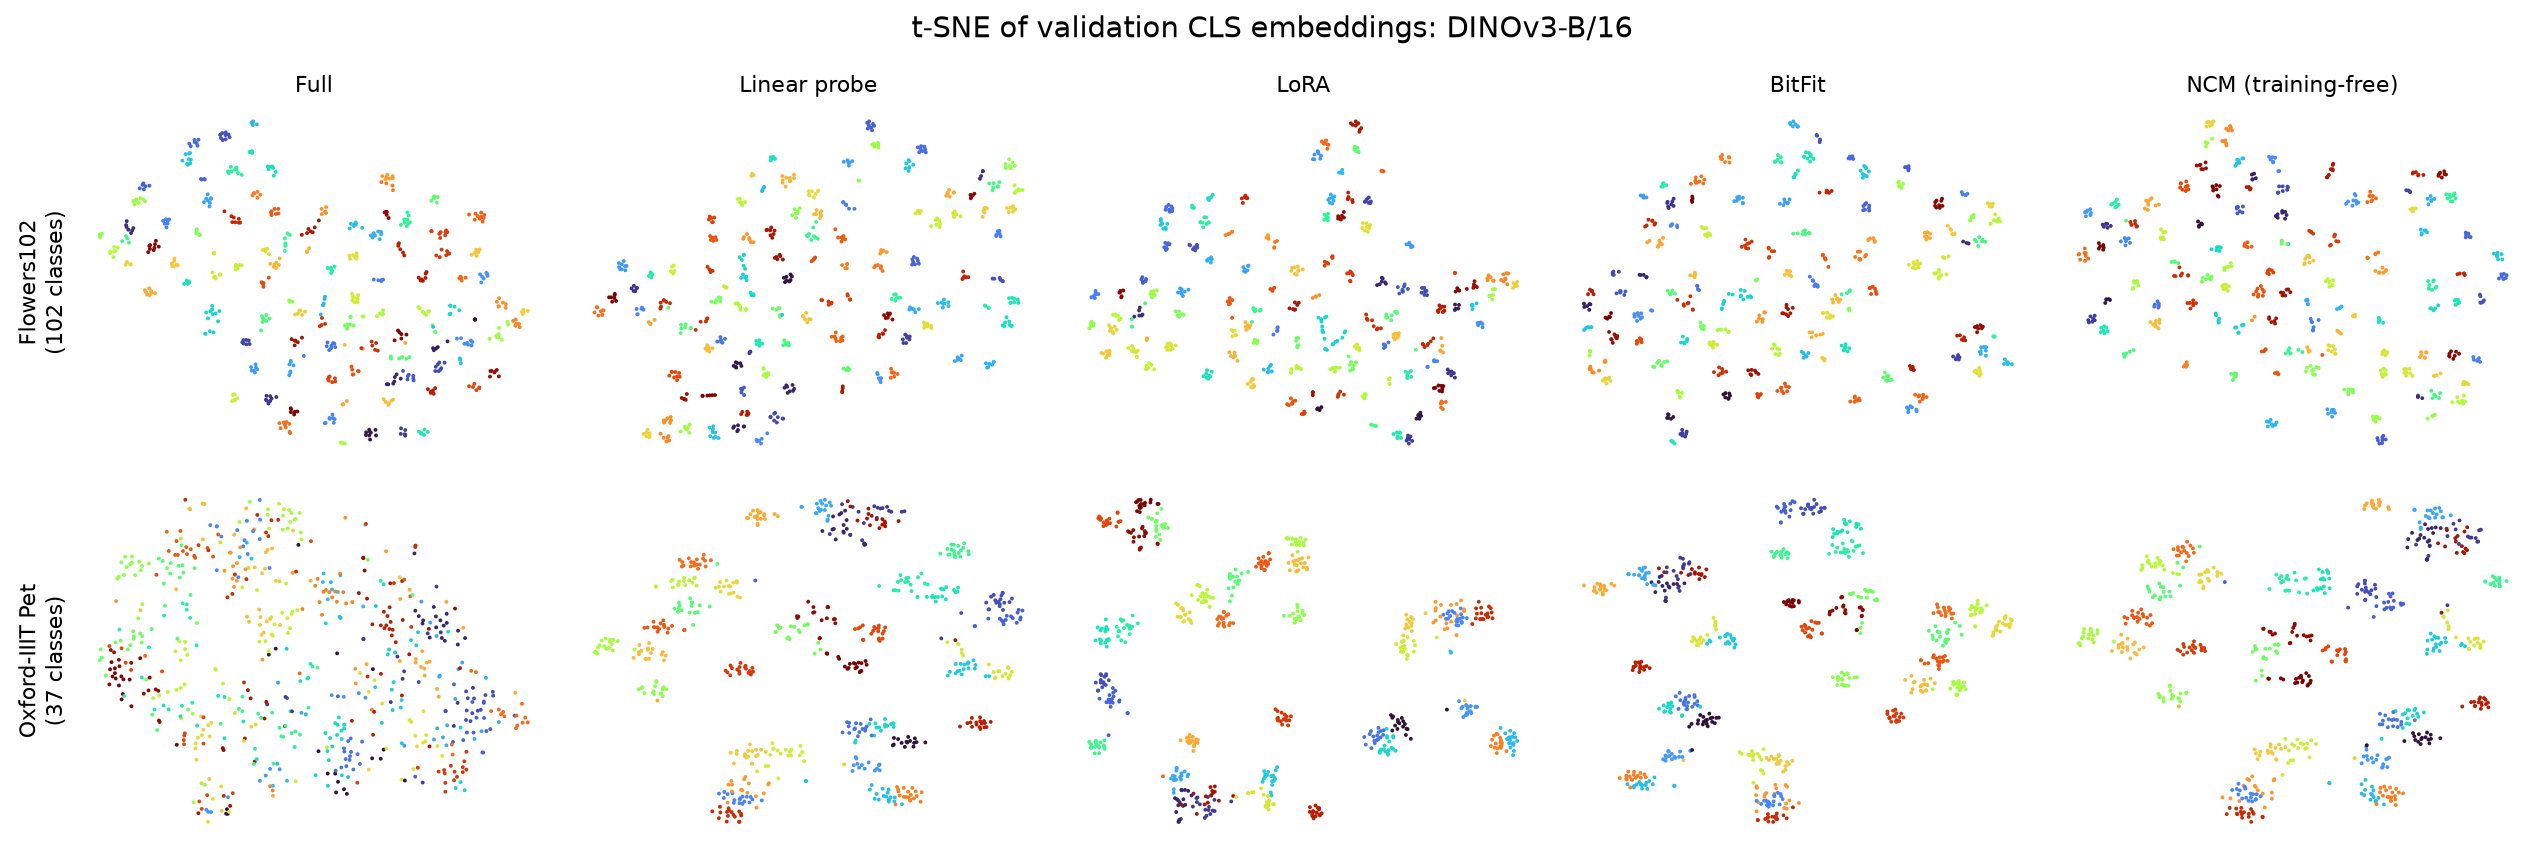
\includegraphics[width=\linewidth]{tsne_dino_v3.png}
  \vspace{-0.18cm}
  {\footnotesize
  \begin{itemize}
    \item Frozen DINOv3 features already form compact clusters under NCM and LP on both datasets; NCM reaches 93.69\% on Pet from those features.
    \item Full fine-tuning on Pet produces an unstructured embedding cloud (46.59\% test), matching the overfit optimisation trace.
  \end{itemize}}
\end{frame}

% --------------------------------------------------------------------------- %
% 20. Observations (accuracy)
% --------------------------------------------------------------------------- %
\begin{frame}[t]{Observations (1/2): Accuracy}
  \begin{columns}[T]
    \begin{column}{0.56\textwidth}
      \small
      \begin{itemize}
        \item \textbf{NCM wins all four combinations}: 98.44--99.71\% on Flowers102 and 91.48--93.69\% on Pet, with zero trainable parameters.
        \item \textbf{Flowers102}: the trained methods are now competitive at 92.00--97.01\%; LoRA leads ViT (96.68\%) and full leads DINOv3 (97.01\%).
        \item \textbf{Oxford Pet}: ViT Full reaches 88.10\% with LoRA 1.5 points behind; DINOv3 Full overfits (46.59\%), while LoRA is the best trained DINOv3 method (84.80\%).
        \item \textbf{Frozen DINOv3 features are strong}: NCM gets 93.69\% on Pet versus 75.90\% for its LP head on the same features.
        \item \textbf{LoRA and BitFit are close on Flowers102} (95.22--96.68\%) but trail full fine-tuning by 1.5--3.9 points on ViT/Pet.
      \end{itemize}
    \end{column}
    \begin{column}{0.42\textwidth}
      \centering
      \scriptsize
      \setlength{\tabcolsep}{3pt}
      \begin{tabular}{lccc}
        \toprule
        Setting & Best & Acc & Runner-up \\
        \midrule
        ViT / Flowers & NCM & 98.44 & LoRA 96.68 \\
        ViT / Pet & NCM & 91.48 & Full 88.10 \\
        DINOv3 / Flowers & NCM & 99.71 & Full 97.01 \\
        DINOv3 / Pet & NCM & 93.69 & LoRA 84.80 \\
        \bottomrule
      \end{tabular}

      \vspace{0.25cm}
      \begin{block}{Reading the table}
        \footnotesize
        Every best result is training-free (NCM). The best trained method is LoRA on ViT/Flowers and DINOv3/Pet, and full fine-tuning on ViT/Pet and DINOv3/Flowers.
      \end{block}
    \end{column}
  \end{columns}
\end{frame}

% --------------------------------------------------------------------------- %
% 21. Observations (efficiency)
% --------------------------------------------------------------------------- %
\begin{frame}[t]{Observations (2/2): Accuracy per Unit of Compute}
  \centering
  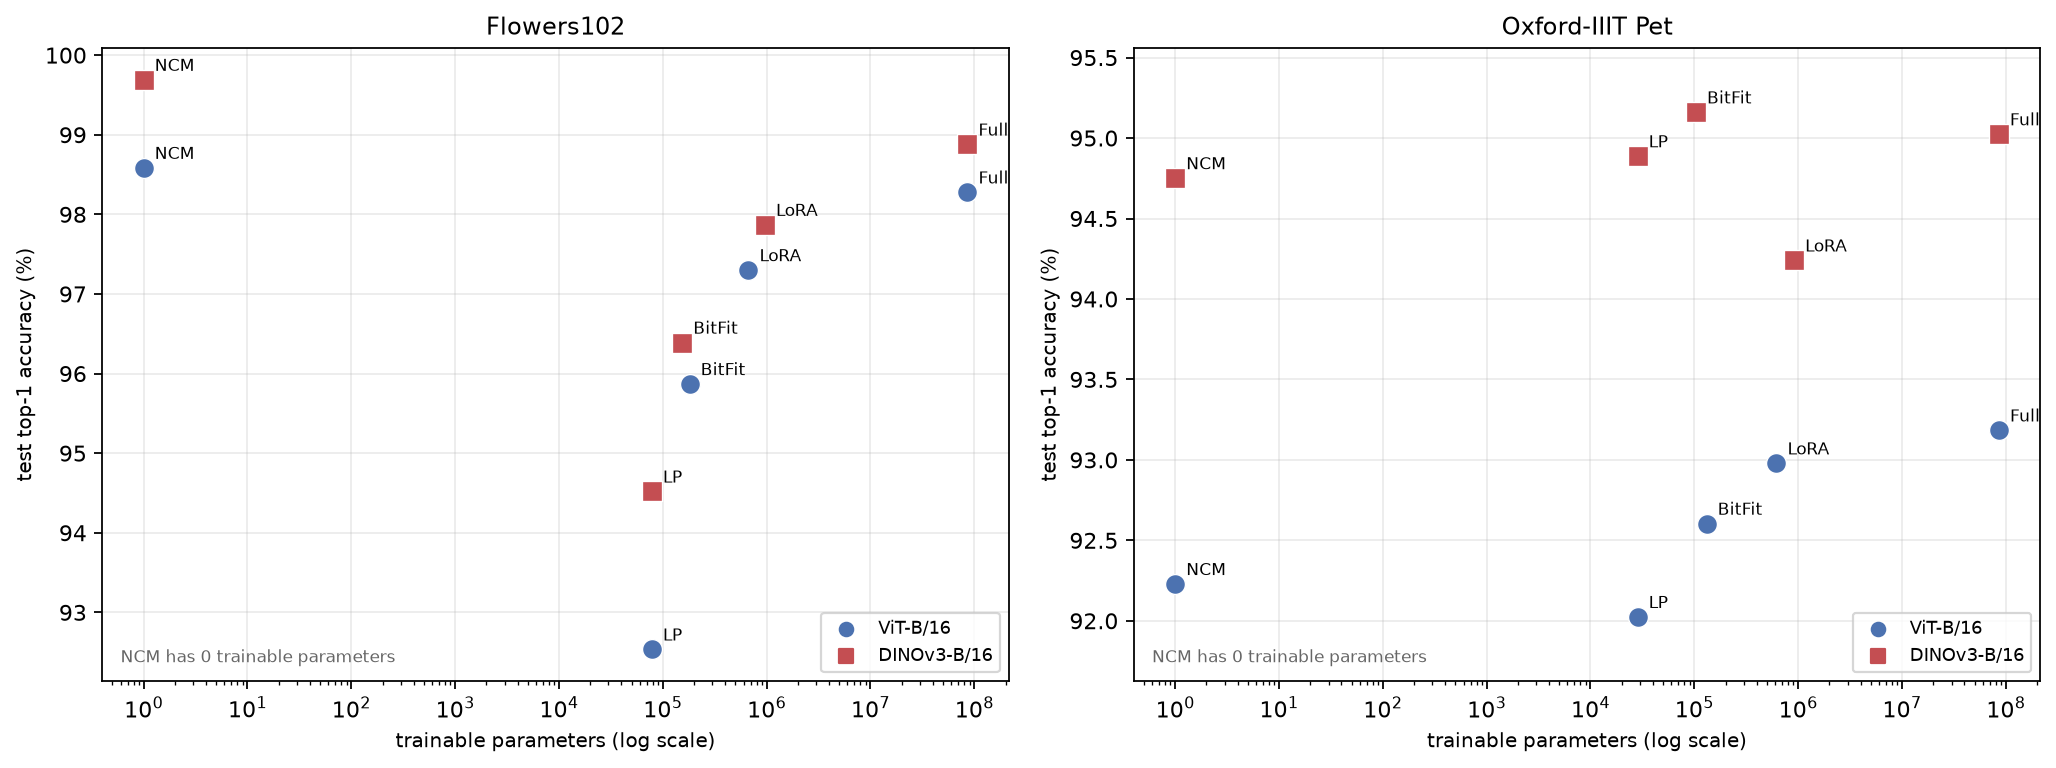
\includegraphics[width=\linewidth,height=0.56\textheight,keepaspectratio]{efficiency.png}
  \vspace{-0.18cm}
  {\footnotesize
  \begin{itemize}
    \item Full fine-tuning costs 254--476\,s and 5.0--7.4\,GB; LP costs 187--267\,s and 0.63--0.71\,GB; NCM costs 6.6--12.8\,s and 0.62--0.70\,GB.
    \item NCM is on the Pareto frontier in all four combinations: it is the most accurate method everywhere at zero trainable parameters.
    \item On Flowers102, DINOv3 NCM reaches 99.71\% in 7.2\,s and 0.70\,GB; on Pet, 93.69\% in 11.4\,s.
    \item Full fine-tuning is never the best overall choice; even on ViT/Pet it is dominated by NCM.
  \end{itemize}}
\end{frame}

% --------------------------------------------------------------------------- %
% 22. Unexpected observations
% --------------------------------------------------------------------------- %
\begin{frame}[t]{Unexpected Observations}
  \footnotesize
  \begin{enumerate}
    \setlength{\itemsep}{2pt}
    \item \textbf{NCM beats every trained method} on both datasets and both backbones: ViT 98.44 vs 96.68 (Flowers) and 91.48 vs 88.10 (Pet); DINOv3 99.71 vs 97.01 (Flowers) and 93.69 vs 84.80 (Pet) --- with zero training and zero trainable parameters.
    \item \textbf{DINOv3 full fine-tuning overfits on Pet}: 46.59\% test while ViT Full reaches 88.10\% on the same 370 images. Train loss 0.156 vs val loss 1.85, and the best checkpoint is epoch 17.
    \item \textbf{Frozen DINOv3 features far outperform their LP head on Pet}: 93.69\% (NCM) vs 75.90\% (LP) on identical features; the head trained on 10 shots is still the bottleneck.
    \item \textbf{10.5$\times$ memory for a much worse result}: DINOv3 Full uses 7.36\,GB vs 0.70\,GB for NCM; on Pet it is 47.1 points less accurate, and on Flowers 2.70 points less.
    \item \textbf{ViT LP is the weakest Flowers102 method} (92.00\%), yet ViT NCM reaches 98.44\% on the same frozen features.
    \item \textbf{DINOv3 Full on Pet has 80.67\% top-5 but 46.59\% top-1}: the right class is often retrieved but ranked poorly; elsewhere top-5 accuracy is 97.68--99.93\%.
  \end{enumerate}
\end{frame}

% --------------------------------------------------------------------------- %
% 23. Test results (1/2): Flowers102
% --------------------------------------------------------------------------- %
\begin{frame}[t]{Test Results (1/2): Flowers102}
  \centering
  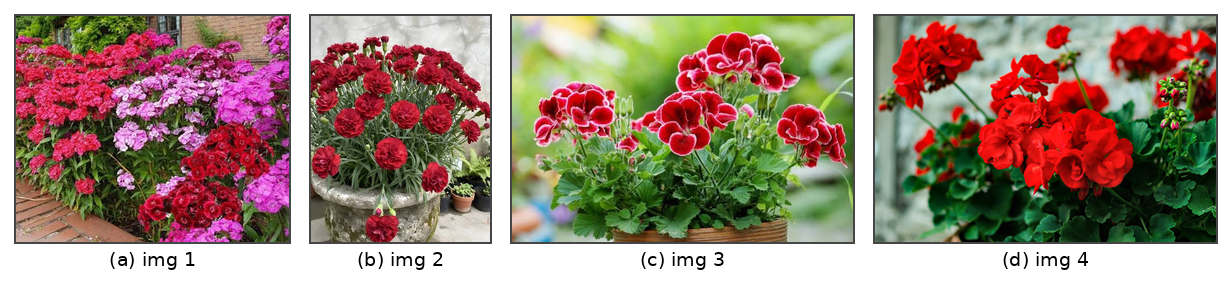
\includegraphics[width=0.94\linewidth,height=0.32\textheight,keepaspectratio]{test_strip_flowers102.png}

  \vspace{0.2cm}
  \renewcommand{\arraystretch}{1.3}
  \setlength{\tabcolsep}{4pt}
  \scriptsize
  \begin{tabular}{lcccccc}
    \toprule
    Image & Ground truth & Full & LP & LoRA & BitFit & NCM \\
    \midrule
    (a) & sweet william & \textcolor{red}{prince of wales feathers} & \textcolor{red}{geranium} & \textcolor{red}{geranium} & \textcolor{red}{geranium} & \textcolor{red}{garden phlox} \\
    (b) & carnation & carnation & \textcolor{red}{californian poppy} & \textcolor{red}{azalea} & \textcolor{red}{californian poppy} & carnation \\
    (c) & pelargonium & \textcolor{red}{wallflower} & \textcolor{red}{geranium} & \textcolor{red}{geranium} & \textcolor{red}{geranium} & \textcolor{red}{geranium} \\
    (d) & geranium & geranium & geranium & geranium & geranium & geranium \\
    \bottomrule
  \end{tabular}

  \vspace{0.08cm}
  {\tiny Red entries are incorrect predictions; all methods are DINOv3-B/16.}

  \vspace{0.18cm}
  {\footnotesize \textbf{Setup:} tested on the trained weights obtained using the different strategies (Full, LP, LoRA, BitFit) and the training-free NCM classifier; these hand-selected images are outside the train, validation, and test splits.}
\end{frame}

% --------------------------------------------------------------------------- %
% 24. Test results (2/2): Oxford-IIIT Pet
% --------------------------------------------------------------------------- %
\begin{frame}[t]{Test Results (2/2): Oxford-IIIT Pet}
  \centering
  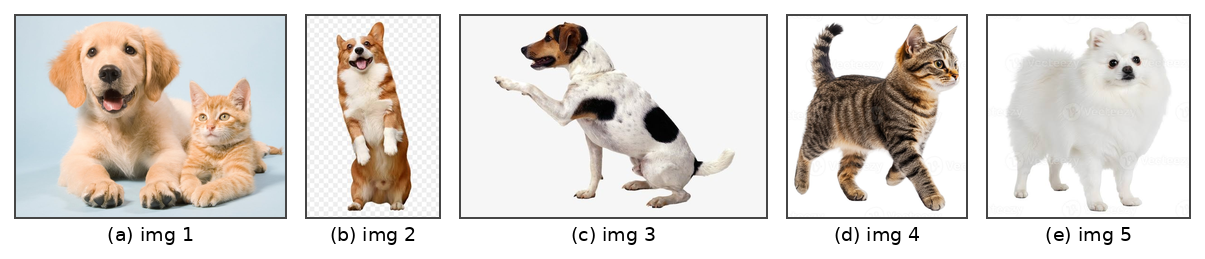
\includegraphics[width=0.94\linewidth,height=0.32\textheight,keepaspectratio]{test_strip_oxfordiiitpet.png}

  \vspace{0.2cm}
  \renewcommand{\arraystretch}{1.3}
  \setlength{\tabcolsep}{4pt}
  \scriptsize
  \begin{tabular}{lcccccc}
    \toprule
    Image & Ground truth & Full & LP & LoRA & BitFit & NCM \\
    \midrule
    (a) & great pyrenees & \textcolor{red}{abyssinian} & \textcolor{red}{german shorthaired} & \textcolor{red}{leonberger} & \textcolor{red}{german shorthaired} & great pyrenees \\
    (b) & shiba inu & \textcolor{red}{saint bernard} & shiba inu & shiba inu & shiba inu & shiba inu \\
    (c) & beagle & \textcolor{red}{sphynx} & \textcolor{red}{english setter} & beagle & \textcolor{red}{english setter} & beagle \\
    (d) & bengal & bengal & \textcolor{red}{abyssinian} & bengal & \textcolor{red}{abyssinian} & \textcolor{red}{egyptian mau} \\
    (e) & pomeranian & \textcolor{red}{ragdoll} & \textcolor{red}{samoyed} & \textcolor{red}{samoyed} & \textcolor{red}{samoyed} & pomeranian \\
    \bottomrule
  \end{tabular}

  \vspace{0.08cm}
  {\tiny Red entries are incorrect predictions; all methods are DINOv3-B/16.}

  \vspace{0.18cm}
  {\footnotesize \textbf{Setup:} tested on the trained weights obtained using the different strategies (Full, LP, LoRA, BitFit) and the training-free NCM classifier; these hand-selected images are outside the train, validation, and test splits.}
\end{frame}

% --------------------------------------------------------------------------- %
% 25. The End
% --------------------------------------------------------------------------- %
\begin{frame}[plain]
  \centering
  \vspace{1.3cm}
  {\Huge\bfseries The End}\\[0.35cm]
  {\Large Questions?}\\[0.9cm]
  \begin{minipage}{0.88\textwidth}
    \begin{block}{Take-home message}
      \centering
      In the low-label regime, the frozen representation matters more than the number of trainable parameters: a training-free NCM classifier is the most accurate method on both datasets and both backbones. With a 20-epoch budget, full fine-tuning and LoRA become competitive on Flowers102 and ViT/Pet, but full DINOv3 fine-tuning overfits the ten-shot Pet training set.
    \end{block}
  \end{minipage}
  \vfill
  {\footnotesize Gundapu Nitish Kumar \quad\textbar\quad Mourya Nandan \quad\textbar\quad CS 6350 TPA-17}
\end{frame}

\end{document}
